\documentclass[10pt]{article}
\usepackage{oxycomps}
\usepackage [english]{babel}
\usepackage [autostyle, english = american]{csquotes}
\MakeOuterQuote{"}
\pdfinfo{
    /Title (A Beginner's Tutorial to GitHub Repositories)
    /Author (Bryanna Hernandez)
}
\title{A Beginner's Tutorial to GitHub Repositories}
\author{Bryanna Hernandez}
\affiliation{Occidental College}
\email{bhernandez2@oxy.edu}

\begin{document}

\maketitle

\section{Introduction}

GitHub is a valuable tool for computer science majors to securely store their files and projects online. However, its complexity often presents high barriers to entry for newcomers. This tutorial aims to dismantle these barriers through a step-by-step introduction to GitHub using Command Line. In this tutorial, beginners should expect to learn the basic commands to skillfully control the relationship between GitHub's four main areas: the Working Tree, the Staging Area, the Local Repository, and the Remote Repository. At the conclusion of this tutorial, beginners will also be given some tips on how to further master GitHub. This tutorial is accurate as of January 2024 and is geared toward the Windows Operating System. 

\section{Creating a Repository}

In GitHub, a repository is a fancy word for a place to store your files and code. GitHub supports two different types of repositories. The first is known as a \textbf{Remote Repository}, which is hosted on GitHub's servers. This type of repository can be accessed from any local machine which means that if you were to lose your computer, for example, you would still be able to access your files. 

Let's start by setting up a remote repository on GitHub's site:

\begin{enumerate}
	\item Go to \url{https://github.com/} and create a profile if you haven't already.
	\item Once logged in, you should be able to see your Dashboard. To the left of the screen there will be a section for "Top Repositories" and a green button called "New". Click this button.
	\item You should see a screen like in Figure\ref{fig:Fig1}, asking you to fill in some data to initialize your repository. While these other fields have useful settings for later projects, for now, title your repository "Tutorial" and click "Create Repository".
\end{enumerate}

Congratulations, you've created your first GitHub remote repository! Next up, we want to transfer this repository to your local machine, known as a \textbf{Local Repository}, through the process of \textbf{Cloning}:

\begin{enumerate}
\item Access your Tutorial repository's page on GitHub. From this screen, there will be a blue section, giving you the option to select between an HTTPS URL or an SSH key. Select HTTPS and copy the URL given. 
\item Open your machine's command terminal and locate the folder you wish to initialize your local repository in.
	\begin{itemize}
	\item For those unfamiliar with command terminal, you can change between folders using  \texttt{cd $<$foldername$>$} .
	\end{itemize}
\item  Clone your repository by typing the command  \texttt{git clone $<$httpslink$>$} .
\end{enumerate}

Double-check that the cloning process worked by using your machine's file explorer. If you see a file called "Tutorial" then congratulations, you have successfully cloned your repository!

\section{Adding Files to Repositories}
Now that you have these two repositories, it's time to make use of them! A README text file is a great first file to add to a repository as it will introduce your project, so let's create one:
 
\begin{enumerate}
\item Open your machine's command terminal and open your Tutorial repository.
\item Create a README text file by typing the command \texttt{Notepad ReadMe.txt} . Your machine should automatically open the application.
\item Edit your README file and save it. For now, it's enough to type something simple like \texttt{hello world!} though in the future, you should aim for your READMEs to be more practical.
\end{enumerate}

You've created your first file for your repository, however, it hasn't yet been uploaded to your local repository. Instead, it was created in what is referred to as a \textbf{Working Tree}. A working tree is an area where you can edit and create files that are useful for your project. However, in order to add files to your directory, you first have to transfer them to the \textbf{Staging Area}: 

\begin{enumerate}
\item In your Tutorial repository, type the command \texttt{git status} . This will bring up all the files within your working tree, which for now, is only your README file. You will see that this file is considered untracked. 
\item Add your file to the staging area by typing the command \texttt{git add ReadMe.txt} .
\item Now check your Tutorial's status once again. You should see that the ReadMe file is now considered a change to be committed. This means it has been successfully added to the staging area. 
	\begin{itemize}
	\item If you ever want to take a file out of the staging area, use the command \texttt{git rm --cached $<$filename$>$} .
	\end{itemize}
\end{enumerate}

Once a file is in the staging area, there is one more step to add it to your local repository. While this may seem excessive, the staging area can be useful for projects with lots of moving parts. In the future, you can add multiple files to the staging area using the command \texttt{git add --all} . This will allow you to move all files to your repository in one step which may be necessary if a part of your project requires multiple files to be updated simultaneously to continue functioning and would break if only one file was uploaded. 

As you may have seen in the last step, adding a file to the local repository is known as \textbf{committing} a file. Let's do that now:

\begin{enumerate}
\item In your Tutorial repository, move your file to the local repository with the command \texttt{git commit -m \char`\"adding ReadMe\char`\"} .
\item Check your git status. If your file was properly committed, you should see that your working tree is clean.
\item To check your commit history, use the command \texttt{git log} . Under a long alphanumerical string, you should see the date and time you pushed the commit, as well as your commit message. 
\end{enumerate}

Committing a file is often viewed as saving a repository, and when you make a lot of commits, it can be useful to differentiate these saves in your commit history by writing yourself a message, such as what was written above in the quotations. In the future, your commit message can be as long or short as you want as long as you include the quotation marks, but you'll thank yourself later when you're searching through your commit history if you keep them practical. 

You've updated your local repository through committing, but updating a remote repository is known as \textbf{pushing} because it pushes your local files to your remote repository. However, you can only push whatever has been committed to your local repository; nothing in the working tree or the staging area can be pushed. 

Let's push our README file to GitHub's remote repository:

\begin{enumerate}
\item In your Tutorial repository, type the command \texttt{git push origin main} . 
	\begin{itemize}
	\item As this is your first time pushing to the remote repository, you may be asked to login to your GitHub account in your browser.
	\end{itemize}
\item In your browser, open your GitHub Tutorial repository. If you were successful, you should now see your README file. Because using a README file is standard practice, you should also be able to see the text within in the file right below, although other files can be accessed by clicking on their names.
\end{enumerate}

The git push command has two important references. The first reference to origin is shorthand for the URL of the remote repository on your GitHub account. In most cases, just git push is enough, but if you wanted to push the files in your local repository to a different remote repository, then you would want to specify. 

The second reference to main specifies which branch of your repository you are pushing to. In simple terms, a \textbf{Branch} is a tag associated with your commit that tells GitHub which version of your project to display to others. Your first commit is by default considered the main branch, but it may be useful in the future to have other branches dedicated to feature experimentation. When a branch is made, it uses the most recent commit of its parent branch, in this case main, as it's jumping off point. Branches allow you to make and save changes to your project without impacting the main version of your project. If you are only working with one branch, it is not necessary to specify in your push commands, but it is good practice!

\section{Adding and Using Branches in Repositories}
Let's make a new branch in your command terminal to demonstrate:

\begin{enumerate}
\item In your Tutorial repository, type the command \texttt{git branch side} . 
\item To confirm this branch has been created, type the command \texttt{git branch} . You should see a list of branches, starting with main and then side. Additionally, the astrix next to main verifies that we are currently working on this branch.
\item To switch branches, type the command \texttt{git switch side} . 
\item Confirm with the command \texttt{git branch} . If you have successfully switched branches, the astrix should be next to the side branch. 
\end{enumerate}

Branches can be named anything, side is just an example. It is best to name a branch something meaningful to you. Just as the main branch can be uploaded to the remote repository, so can a side branch. Now, let's edit the side branch further demonstrate how it works:

\begin{enumerate}
\item In your Tutorial repository, open your README file using the command \texttt{Notepad ReadMe.txt} . You'll notice that this is the same command we used to create the file.
\item Edit your README file by typing on the second line. Again, a simple sentence will do, but be sure not to edit the first line for now. Save your file.
\item Add this file to the staging area and commit the file to your local repository using the commands given above.
\item Now check your commit history. For now, only take note of the red tag attached to your commits. 
\begin{itemize}
\item Your commit history should look similar to Figure\ref{fig:Fig2}.
\end{itemize}
\item Push your new changes to the remote repository. 
\item Now check your commit history. This time, take note of the green and blue tags attached to your commits as well as the red tags.
\begin{itemize}
\item Your commit history should now resemble Figure\ref{fig:Fig3}.
\end{itemize}
\item Now switch your branch to the main branch and check your commit history for a third time.
\end{enumerate}

The red tags on your commits reflect the last $pushed$ commit of a branch. You should have noticed that on the first check, the side branch did not have a red tag because it had never been pushed. However, on the second check, it was given a red tag to reflect the updates made to the remote repository.

The green tags on your commits are the names of your branches, though it is important to note that these tags will only be attached to the most recent commit within that branch. 

The blue tag that says "Head -$>$" indicates the last commit of the branch that you are $currently$ working in. When you first checked your commit history, it would have pointed to the green side tag, and now it should be pointing to main. In fact, when switching your commit branch to main, you might have no longer seen your side branch commit history. It is good to note that branches have a hierarchy and will only show the commit log of its own branch and the parent branch(es) that were created before it.    

Additionally, if you return to the tutorial repository on your GitHub website, you will see a button labeled main next to text that clarifies the number of branches pushed to your remote repository. If you click on the main button and select your side branch, you will be able to see the changes reflected to your README file. 

\section{Merging Branches}

In the same way that you can create branches within your project, you can also combine your branches back into one. This process is known as \textbf{merging} and depending on the layout of your files, it may not succeed. First, let's demonstrate a successful merge:

\begin{enumerate}
\item In your Tutorial repository, ensure that you are on the main branch, this is the branch that will remain after the merger. 
\item To merge branches, use the command \texttt{git merge side} .
	\begin{itemize}
	\item A merged branch is automatically committed to the local repository. 
	\end{itemize}
\item Push these changes to your remote repository. 
\end{enumerate}

If you check your changes on the GitHub website, you should see that your README file in the main branch is exactly the same as the file in the side branch. This means it was successful. However, in a merge, the side branch doesn't disappear, it only pushed its changes to the main branch. You are still able to edit, stage, commit, and push files in the side branch without affecting the main branch. 

Now let's attempt an unsuccessful merge, known as a \textbf{merge conflict}:

\begin{enumerate}
\item In your Tutorial repository, open the README file and edit the first line to say "hello world 1." Save the file.
\item Add this file to the staging area and commit the file. 
\item Switch to your side branch.
\item Open the README file, and this time, edit the first line to say "hello world 2". Save your file.
\item Add this file to the staging area and commit the file. 
\item Switch back to the main branch.
\item Use the command \texttt{git merge side} and attempt to merge the two branches.
\end{enumerate}

This type of merging triggers a merge conflict and requires user action in order to complete the merge. A merge conflict happens when attempting to merge a file with competing changes on one line. In this example, the computer is unable to decide which number to keep after hello world and will not allow you to switch branches until the conflict is resolved. Let's attempt to resolve the conflict:

\begin{enumerate}
\item On the main branch, open the README file. 
	\begin{itemize}
	\item You should see an text file that looks similar to Figure\ref{fig:Fig4}. 
	\end{itemize}
\item Edit the file so that it says "hello world 1" on the first line and is blank on the other lines. Save the file.
\item Stage and commit the file. 
\item Push the file to the remote repository. 
\end{enumerate}

In this example solving a merge conflict is a simple as editing the text file. However, in more complicated merge conflicts, you may be required to edit multiple files to resolve the conflict. 

\section{Pulling and Stashing Changes}

We have covered the basics of pushing local repository data to remote repositories, but there is also a method of transferring remote repository data to local repositories. This process is known as \textbf{pulling}, and can be extremely useful when working on a project with collaborators. Let's go through this process together:

\begin{enumerate}
\item On the GitHub website, in your remote repository under the main branch, click on the dropdown "Add file" button and choose "Create new file".
\item Title this new file "PullFile.txt", enter some file contents, and commit the file directly to the main branch.
	\begin{itemize}
	\item When committing files on the GitHub website, staging is not required, and the extended description box allows you to write messages for the commit history.
	\end{itemize}
\item Return to our Tutorial repository in the command terminal and use the command \texttt{git pull origin main} .
	\begin{itemize}
	\item The references in this command work the same as in the pushing command. 
	\end{itemize}
\end{enumerate}

You can verify files have been pulled by checking the commit history or by opening the file yourself. However, whenever changes are pulled from the remote repository, this can overwrite any work that is in your working tree or staging area. Therefore, it can be useful to temporarily save your changes before pulling to then restore your work later in a process known as \textbf{stashing}. Let's simulate this situation:

\begin{enumerate}
\item In your remote repository, create and commit a new file to the main branch titled "NewPull.txt".
\item In the command terminal, in the main branch, open, edit, and save your README file. Do NOT stage or commit this file.
\item Now stash your README file with the command \texttt{git stash} .
\item Use the command \texttt{git stash list} . You should see an item titled stash@\{0\}. This means you have properly stashed your files. 
\item Reopen your README file and verify that the edits you made are gone.
\item Use the pull command to download your NewPull.txt file.
\item Use the command \texttt{git stash pop} to restore the edits to your README file. 
\item Open your README file and verify that the edits have returned.
\end{enumerate}

In this situation, you were able to download the NewPull file without losing your edits in your README file. Best practices advise you to only have one stashed edit at a time and to only use it in temporary situations. Other reasons entail wanting to stash work on one branch to go work on another branch for a change of pace, or to reduce the possibility for merge conflicts. Typically, it is simpler to commit files, but it is up to your judgement to decide when it is necessary to stash files.

\section{Final Words}

GitHub's complexity is somewhat infamous in the tech community. Therefore, while I hope that this tutorial has been a useful jumping off point, there are other great sources of documentation such as on \url{https://git-scm.com/} and the forums on \url{https://stackoverflow.com/} which have answered thousands of beginners' questions regarding GitHub. I encourage all users of this tutorial to seek out online resources whenever they encounter confusion, and above all else, happy coding!

\begin{figure}[t]
    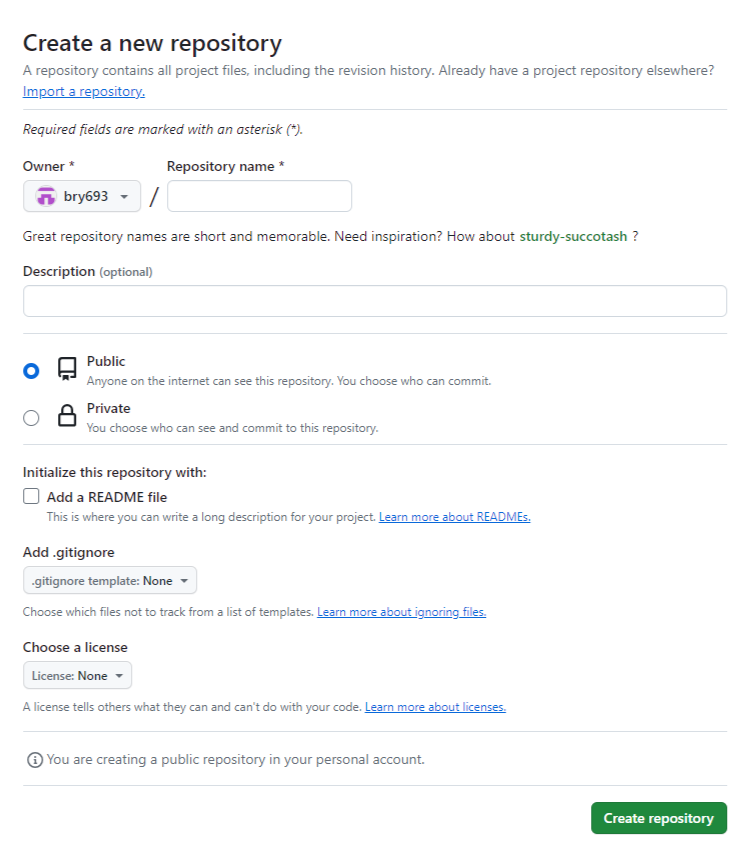
\includegraphics[width=.75\linewidth]{fig1.png}
\centering    
\caption{
        The repository initialization screen, as an image.
    }
    \label{fig:Fig1}
\end{figure}

\begin{figure}
    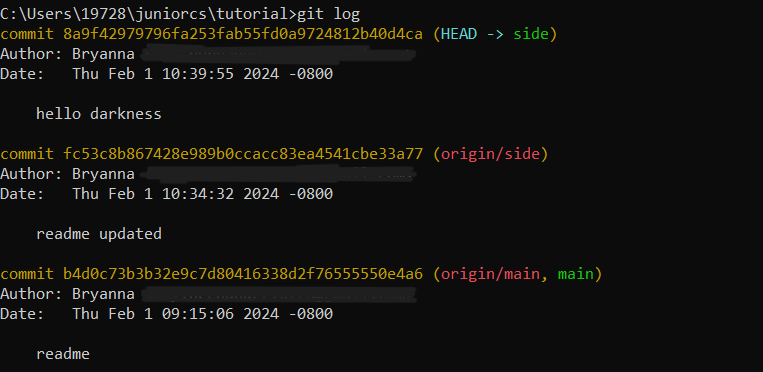
\includegraphics[width=.6\linewidth]{before.png}
\centering
    \caption{
        Commit history before pushing the side branch.
    }
    \label{fig:Fig2}
\end{figure}

\begin{figure}
    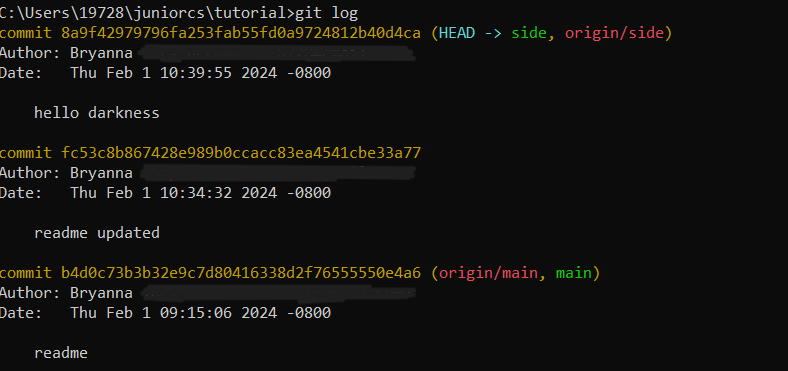
\includegraphics[width=.6\linewidth]{after.png}
\centering
    \caption{
        Commit history after pushing the side branch.
    }
    \label{fig:Fig3}
\end{figure}

\begin{figure}
    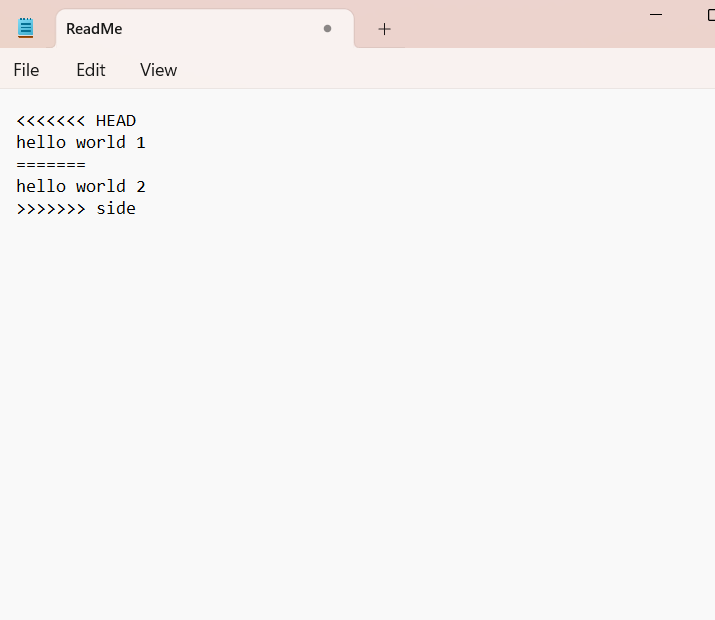
\includegraphics[width=.6\linewidth]{conflict.png}
\centering
    \caption{
        README file experiencing a merge conflict.
    }
    \label{fig:Fig4}
\end{figure}

\end{document}

 
